% \documentclass[12pt]{article} %ordinary compilation
% %\documentclass[aap]{imsart} % to approximate no pages via AOAS template
% \usepackage{setspace}  %comment out if using imsart
% %\arxiv{1403.5478}
%\usepackage{bm}
%\usepackage{subfigure} % NB: subfigure package has been depracated
%in favor of subcaption. But we don't presently seem to need either one.
% above is workaround for Aquamacs bug, see https://groups.google.com/forum/#!topic/aquamacs-devel/r9iaih8rsAg
\usepackage{fullpage}
\usepackage{wrapfig}
\usepackage{enumerate}
\usepackage{graphicx}
\usepackage{graphics}
\usepackage{comment}
\usepackage{amsmath,amssymb,amsfonts,amsthm,amsbsy}
\usepackage{stmaryrd} %bbm,
\usepackage{verbatim}
\usepackage[authoryear]{natbib}
\usepackage{soul}
\usepackage{multirow}
\usepackage{makecell}
\usepackage{bm}
\usepackage{hyperref}
\hypersetup{colorlinks=true,
    linkcolor=blue,
    filecolor=blue,
    citecolor=black,
    urlcolor=cyan}
\usepackage{xr}
%\usepackage{mathabx}
%\usepackage{filecontents}
%\usepackage{bibentry}
%\usepackage{hanging}
%\usepackage{apacite}
%\pdfminorversion=4



\newcommand{\maria}{Maria}
\newcommand{\TildeTheta}{\hat{\theta}}
\newcommand{\InfPar}[1]{\ensuremath{{#1}_{\infty}}}
\newcommand{\thetaInf}{\InfPar{\theta}}
\newcommand{\IC}[3][\hat\theta]{\mathrm{IF}_{#1}(#2, #3)}
\newcommand{\bty}{\mathbf{y}_H}
\newcommand{\btY}{\mathbf{Y}_H}
\newcommand{\tyi}{{y}_{Hi}}
\newcommand{\tYi}{{Y}_{Hi}}
\newcommand{\xch}{\check{X}}
\newcommand{\g}{g}
\newcommand{\ych}{e}
\newcommand{\Ych}{\ensuremath{E}}
\newcommand{\dt}[3][\theta]{\ensuremath{e_{#1}(#2| {#3})}}
\newcommand{\indicator}[1]{\ensuremath{\mathcal{I}\left[#1 \right]}}
                                %alternatives:
                                % {\ensuremath{\llbracket #1 \rrbracket}} % or \mathbbm{1}_{\left\{ {#1} \right\} }
                                % or maybe \chi_ instead of 1_
%\newcommand\independent{\protect\mathpalette{\protect\independenT}{\independent}}
\newcommand{\independent}{\perp}
\newcommand\hsg{\texttt{hsgrade\_pct}}
\newcommand{\hyp}{H_{\tau_0}}
\newcommand{\ychphib}{\boldsymbol{\check{Y}_{\phi_0}}}
\newcommand{\ychphi}{\check{Y}_{\boldsymbol{\phi_0}i}}
\newcommand{\PP}{\mathrm{Pr}}
\newcommand{\EE}{\mathbb{E}}
\newcommand{\var}{\mathrm{Var}}
\newcommand{\cov}{\mathrm{Cov}}
\newcommand{\htO}{H_{\tau_0}}
\newcommand{\tht}{\tilde{H}_{\tau_0}}
\newcommand{\resid}{E}
\newcommand{\meanDiffT}{T_{\tau}} 

\def\independenT#1#2{\mathrel{\rlap{$#1#2$}\mkern2mu{#1#2}}}
\newtheorem{prop}{Proposition}
\newtheorem{lemma}{Lemma}

\newenvironment{ass}[2][Assumption]{\begin{trivlist}
\item[\hskip \labelsep {\bfseries #1}\hskip \labelsep ({\bfseries #2}).]}{\end{trivlist}}




% \externaldocument{rd-aoas}
% \title{Limitless Regression Discontinuity:\\ supporting mathematics
%   and computations}
% \begin{document}
% \maketitle

% AOAS-specific:
% \begin{aug}
% \author{\fnms{Ben B}
%   \snm{Hansen}\thanksref{t2,m2}\ead[label=e2]{bbh@umich.edu}}
% \and
% \author{\fnms{Adam C} \snm{Sales}%\thanksref{t1,m1}\ead[label=e1]{asales@utexas.edu}}
% \thanksref{m1}\ead[label=e1]{asales@utexas.edu}}



% % \thankstext{t1}{The authors thank Susan
% %     Dynarski, Roc\'{i}o Titiunik, Matias Cattaneo, Guido Imbens, Brian Junker,
% %     Justin McCrary, Walter Mebane, Kerby Shedden, Jeff Smith, the participants in the
% %     University of Michigan Causal Inference in Education Research
% %     Seminar and anonymous reviewers for helpful suggestions.}
% \thankstext{t2}{This research was supported by the Institute of
%   Education Sciences, U.S. Department of Education (R305B1000012), the
%   U.S. National Science Foundation (SES 0753164) and an NICHD center
%   grant (R24 HD041028).  Any opinions, findings, and conclusions or
%   recommendations expressed in this material are those of the
%   authors.}
% \runauthor{Hansen \& Sales}

% \affiliation{University of Michigan\thanksmark{m2} and University of Texas College of Education\thanksmark{m1}}

% \address{University of Texas College of Education\\
% SZB 536C\\
% 1912 Speedway, Stop D5000\\
% Austin, Texas 78712\\
% \printead{e1}\\
% }

% \address{Department of Statistics\\
% 445F West Hall\\
% University of Michigan\\
% Ann Arbor, MI 1107\\
% \printead{e2}}

% \end{aug}


% \runtitle{Limitless RD}
%\setcounter{equation}{6}

\doublespacing

\appendix
\begin{comment}
\section{Higher Order Polynomials in RDD Analysis: A Simulation Study}\label{apnd:poly-sim}

        \begin{table}[ht]
\centering
\begin{tabular}{cr|lllll|lllll|l }
  \hline
&& \multicolumn{5}{c|}{Limitless} &  \multicolumn{5}{c|}{OLS} &\makecell[c]{Local\\Linear}  \\
 \multicolumn{2}{r|}{Polynomial Degree}&1&2&3&4&5&1&2&3&4&5& n/a  \\
\hline
\hline
\multirow{ 2 }{*}{ Linear }& bias &0.00&0.00&0.00&0.00&0.00&0.00&-0.01&0.02&0.30&-1.70&0.01\\
& RMSE &0.23&0.23&0.31&0.31&0.37&0.30&1.11&4.68&21.58&106.41&0.48\\
\hline
\hline
\multirow{ 2 }{*}{ Anti-Sym }& bias &-0.63&-0.63&-0.03&-0.03&0.12&-0.64&1.68&1.76&-9.02&-9.38&-0.02\\
& RMSE &0.67&0.67&0.30&0.30&0.38&0.71&2.00&5.04&23.53&106.12&0.50\\
\hline
\hline
\multirow{ 2 }{*}{ Sine }& bias &1.16&1.16&0.17&0.17&0.02&1.16&-2.63&-2.18&1.84&0.17&0.08\\
& RMSE &1.18&1.18&0.35&0.35&0.36&1.20&2.86&5.20&21.45&103.41&0.54\\

 \hline
\end{tabular}
\caption{Results from 5000 simulations of polynomial specifications for RDD analysis, using MM-estimation, OLS or local linear regression. Data generating models were as depicted in Figure~\ref{fig:dgms}, with $t_{3}$ errors; sample size for all runs was 500, and there was no treatment effect.}
\label{tab:poly}
\end{table}


\begin{figure}
\centering
% chunk below  generates figure/dgms-1.pdf , but also includes
% unwanted warnings in latex file.  To regenerate dgms-1.pdf,
% set eval to TRUE, comments out the \includegraphics{} and compile;
% then come back and reset it to FALSE
%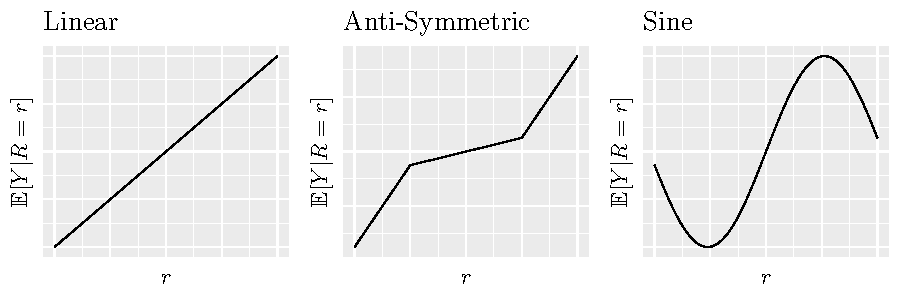
\includegraphics[width=\maxwidth]{figure/dgms-1}
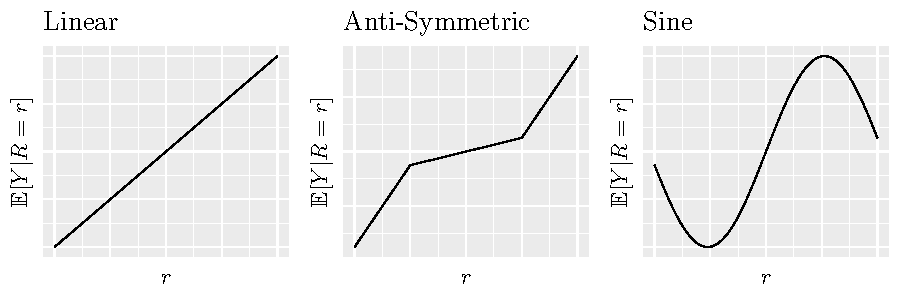
\includegraphics[width=0.9\textwidth]{figure/dgms-1}
\caption{Data generating models for polynomial simulation.}
\label{fig:dgms}
\end{figure}

When $\EE[Y|R=r]$ may not be linear in $r$, flexibility in the
$\mu_{\bm{\beta}}(R)$ function takes on added importance.
% Though higher-order polynomials in $R$ offer that flexibility,
% \citet{gelmanImbens} argue against using them in RDD settings, in part
% because they magnify the leverage of outliers.
% However, robust regression may alleviate this concern.
We ran an additional simulation to explore the potential of robust
polynomial regression to mitigate influence, as discussed in
\S~\ref{sec:test-hypoth-no} above, while adding flexibility
to the specification of the $Y_{C}$ on $R$ regression.
We compared limitless RD analysis, with $\mu_{\bm{\beta}}$ a polynomial in $R$ with
degree 1, 2, 3, or 4, to analogous estimates from OLS.
In the OLS regressions, we followed the advice of \citet[e.g.][p. 318]{lee2010regression} and
included interactions between the $R$-polynomial and $Z$.
Finally, we compared these methods to local-linear regression with the
bandwidth of \citet{imbens2012optimal}.
The OLS and limitless methods used the entire range of data.
We simulated data sets of size $n=500$ by drawing $R$ and $\epsilon$
from Uniform $(-1,1)$ and  $t_3$ distributions respectively, then
adding $\epsilon$ to one of the three functions of $R$ shown in
Figure~\ref{fig:dgms} to form $Y_{C}$.
%Additional simulations with standard normal errors are displayed in
%Appendix B.

Table~\ref{tab:poly} displays the results.
For both limitless and OLS methods, linear and quadratic specifications suffered severe inflation of type-I
error under either non-linear data generating model.
With a cubic or quartic
specification, the limitless method achieved nominal
levels, whereas OLS's were slightly inflated.
OLS and robust regression sharply diverge in the quality of their
point estimates: the root mean squared error (RMSE) of OLS estimation
increases rapidly with polynomial degree, but robust regression's does not.
With the robust regression-based method but not with OLS, increasing
the degree of the polynomial improved accuracy of testing and
estimation in the presence of non-linearity.

The local linear model does not employ higher-order global
polynomials. It fared better than OLS, but worse than cubic or quartic robust regression.

\end{comment}
\section{Large-sample randomization inference in RCTs}
Section~\ref{sec:randProc} %of \citet{lrdauthors:main}
discusses
$t_{u}(\mathbf{Y}, \mathbf{Z})$, the two-sample $t$ statistic without
pooling of variances as considered by Neyman, in RCTs. The discussion
is in the context of a fixed total sample size $n$ and of conditioning on
\begin{equation*}
\mathcal{N} = \sigma(\tilde{\mathbf{Y}}_{T}, \tilde{\mathbf{Y}}_C,
\mathbf{D}_{T}, N_{0}, N_{1})\quad \text{or} \quad \mathcal{N}^{*} = \sigma(\tilde{\mathbf{Y}}_{T}, \tilde{\mathbf{Y}}_C,
\mathbf{D}_{T}),
\end{equation*}
where $\tilde{\mathbf{v}} = \mathbf{v} - \bar{v}$ and
$N_{j}=\sum_{i=1}^{n} \indicator{Z_{i}=j}$, $j=0,1$.  Since neither
$\bar{Y}_T$ nor $\bar{Y}_C$ is observed, $\tilde{\mathbf{Y}}_{T}$ and
$\tilde{\mathbf{Y}}_C$ are unobserved, despite ${\mathbf{Y}}_{T}$ and
${\mathbf{Y}}_C$ being partly observed; after conditioning on
$\mathcal{N}$ or $\mathcal{N}^{*}$, $\tilde{\mathbf{y}}_{T}$ and
$\tilde{\mathbf{y}}_C$ are fixed but unobserved constants.

Elsewhere in Section~\ref{sec:randProc} conditioning on
$\mathcal{F}=\sigma(\mathbf{Y}_{C}, N_{0}, N_{1})$ is discussed, but without
corresponding claims about asymptotics under that conditioning;
accordingly it is not discussed further in this supplement.  Later,
however, in
Section~\ref{sec:theMethod} and following, the conditioning is with respect to
\begin{equation} \label{eq:1}
\mathcal{F}^*_{n}=\sigma\left[ \dt[\thetaInf]{\mathbf{Y}_{C}}{
    \mathbf{R}},
\mathbf{D}_{T},  \{(Y_{Ti},
Y_{Ci}, D_{Ti}, R_{i})\indicator{{R}_{i} \not\in
  \mathcal{W}}\}_{i=1}^{n}\right],
\end{equation}
a sigma field resembling $\mathcal{F}$ in bearing
information about $Y_C$s but not $Y_T$s but that, in contrast to
$\mathcal{F}$ but in similarity to $\mathcal{N}^*$, does not carry
information about the sizes of the treatment and control groups
(within $\{i : R_{i} \in \mathcal{W}\}$).
In~\eqref{eq:1}, conditioning on full information about subjects $i$
whose $R$ values fell outside $\mathcal{W}$ is a formal reflection of
those subjects' removal from the analytic sample.

Recall from \S~\ref{sec:rand} %\citet[\S~\ref{sec:rand}]{lrdauthors:main}
that we work
under the assumptions of non-interference, the exclusion restriction
and monotonicity (of $(D_{C}, D_{T})$).  In varying degree, the
sections that follow place additional assumptions bounding $Y_{T}$,
$Y_{C}$ or transformations of them.


\subsection{Normality of $t_{u}(\mathbf{Y}_{H}, \mathbf{Z})$
} \label{apnd:RICLT}




% For simplicity we argue conditionally upon $\mathcal{N}_{\infty} =
% \cup_{n\geq 1} \mathcal{N}_{n}$.  Conditional on $\mathcal{N}_{n}$,
% $\{(\tilde{Y}_{Ti(n)}, \tilde{Y}_{Ci(n)}, D_{Ti(n)}, D_{Ci(n)}): i=1, \ldots, n; n\}$ can be considered a triangular array
% $\{(\tilde{y}_{Ti(n)}, \tilde{y}_{Ci(n)},  d_{Ti(n)}, d_{Ci(n)}): i=1, \ldots, n; n\}$ of fixed
% constants, and $(N_{1(n)}, N_{0(n)})$ can also be considered fixed.
% We shall abuse notation by writing
% $Y_{Ti}, Y_{Ci}, \tilde{y}_{Ti}, \tilde{y}_{Ci},
% d_{Ti}, d_{Ci}$,
% $n_{1}$ and $n_{0}$ for
% $Y_{Ti(n)}, Y_{Ci(n)}, \allowbreak \tilde{y}_{Ti(n)},
% \tilde{y}_{Ci(n)}, \allowbreak  d_{Ti(n)}, d_{Ci(n)}$,
% $n_{1(n)}$ and $n_{0(n)}$ respectively.

First, fix $H: Y_T = Y_C + \tau_0 D_T$ and write
\begin{equation}
  \label{eq:yhc}
  {Y}_{HC} = {Y}_{T} - {D}_{T}\tau_{0}\quad
  \text{and}  \quad Y_{H} = ZY_{HC} + (1-Z)Y_{C},
\end{equation}
 so that for each $i$  ${Y}_{HC i}$ is the  $y_{C}$-value that would be
 reconstructed from data $(y_{Ti}, d_{Ti})$ under $H$, if $(y_{Ti},
 d_{Ti})$ rather than $y_{Ci}$ were observed, whereas $\mathbf{y}_{H}$ is the reconstruction of $\mathbf{y}_{C}$
 according to $H$ based on those data that were actually observed.  Thus $\mathbf{Y}_{HC} \equiv \mathbf{Y}_{C}$ if $H$ is true, but not otherwise. To focus ideas suppose $(Y_{HC}, Y_{C})$ to be bounded.

Second, finite population sampling theory entails as $n_{0}$
and $n_{1}$ increase, the difference between \eqref{eq:sudef}'s
$\mathrm{SE}_{u}^2$, a random variable, and the $\mathcal{N}^{*}$-constant
$s^{2}(\tilde{\mathbf{y}}_{T(n)} - \tau_0\mathbf{d}_{T(n)})/n_1 +
s^{2}(\tilde{\mathbf{y}}_{C(n)})/n_0$,
where $s^{2}(\mathbf{v}) = (n-1)^{-1}\sum (v_{i} - \bar{v})^{2}$,
tends to 0, at rate $o_P[\min(n_0, n_1)^{-1}]$.
For $j=0$ or $1$ and for any $\mathbf{v} = (v_{1}, \ldots, v_{n})$,  $\EE
[s^{2}_{Z=j}(\mathbf{v}) | N_{j}=n_{j}] =
s^{2}(\mathbf{v})$ \citep[Thm.~2.4]{cochran:1977}, while $\var
[s^{2}_{Z=j}(\mathbf{v}) | N_{j}=n_{j}] =$
$$\frac{n_{j}^{2}}{(n_{j}-1)^{2}}\frac{n_{(1-j)}}{n+1}\left\{
\frac{1}{n_{j}}\left(1 - \frac{1}{N} \frac{n_{j}+1}{n_{j}-1}\right)
\kappa_{4}(\mathbf{v}) +
  \frac{2}{n_{j}-1}s^{4}(\mathbf{v}) \right\},$$
where $\kappa_{4}(\mathbf{v})$ denotes the fourth cumulant of
$\mathbf{v}$ \citep[ex. 12.11, p.422]{kendallStuartOrd87}.  Boundedness of $(Y_{HC}, Y_{C})$ entails boundedness for
$s^{4}(\tilde{\mathbf{y}}_{T} - \tau_0\mathbf{d})$, $\kappa_{4}(\tilde{\mathbf{y}}_{T(n)} - \tau_0\mathbf{d})$,
$s^{4}(\tilde{\mathbf{y}}_{C})$, and $\kappa_{4}(\tilde{\mathbf{y}}_{C})$, forcing
the conditional variances of $s^{2}_{Z=1}(\tilde{\mathbf{y}}_{T} - \tau_0\mathbf{d})$ and
$s^{2}_{Z=0}(\tilde{\mathbf{y}}_{C})$ to be  $O(n_0^{-1})$ and $O(n_1^{-1})$,
respectively, so that $s^{2}_{Z=1}(\tilde{\mathbf{y}}_{T} - \tau_0\mathbf{d}) - s^{2}(\tilde{\mathbf{y}}_{T} - \tau_0\mathbf{d})$ and $s^{2}_{Z=0}(\tilde{\mathbf{y}}_{C})-s^{2}(\tilde{\mathbf{y}}_{C})$ tend in probability to 0 as $n_0$ and $n_1$ increase without bound.  To connect this to \eqref{eq:sudef}'s definition of $\mathrm{SE}_u^2$ as the sum of
$s^{2}_{Z=1}({\mathbf{y}}_{T} - \tau_0\mathbf{d})/n_1$ and
$s^{2}_{Z=0}({\mathbf{y}}_{C})/n_0$, observe that $s^{2}_{Z=j}(\tilde{\mathbf{y}}_{C}) = s^{2}_{Z=j}({\mathbf{y}}_{C})$ and $s^{2}_{Z=j}(\tilde{\mathbf{y}}_{T} - \tau_0\mathbf{d}) = s^{2}_{Z=j}({\mathbf{y}}_{T} - \tau_0\mathbf{d})$, $j=0$ or 1.

 Third, as shown by e.g. \citet{samii2012equivalencies},
$$
\var(\overline{({y}_{H})}_{Z=1} - \overline{({y}_{H})}_{Z=0} |
\mathcal{N}) \leq
s^{2}(\tilde{\mathbf{y}}_{T(n)} - \tau_0\mathbf{d}_{(n)})/n_{1}
+ s^{2}(\tilde{\mathbf{y}}_{C(n)})/n_{0} ;
$$
since $\mathcal{N} \subseteq \mathcal{N}^{*}$, a similar inequality
holds with conditioning on $\mathcal{N}^{*}$ rather than
$\mathcal{N}$.  Combining this with the previous solution, the ratio of
$\mathrm{SE}_u^2$ to $\var(\overline{({y}_{H})}_{Z=1} - \overline{({y}_{H})}_{Z=0} |
\mathcal{G})$, $\mathcal{G} = \mathcal{N}$ or $\mathcal{N}^{*}$,
converges to $\nu \leq 1$.


It remains to show that  $\overline{({y}_{H})}_{Z=1} -
\overline{({y}_{H})}_{Z=0}$ is asymptotically Normal.  We may assume
that $\PP(Z_{i}=j) > 0$, $j=0$, 1.  Under
conditioning on $\mathcal{N}^{*}_{n} =
\sigma\left(\{\tilde{Y}_{Ti}\}_{i=1}^{n},
  \{\tilde{Y}_{Ci}\}_{i=1}^{n}, \{D_{Ti}\}_{i=1}^{n} \right)$,
\begin{equation*}
\sum_{i=1}^{n} \left\{\frac{\indicator{Z_{i}=1}}{\PP({Z_{i}=1})} [Y_{HC i} -
\EE(Y_{HC i})] \, \text{and}\, \frac{\indicator{Z_{i}=0}}{\PP({Z_{i}=0})} [Y_{C i} -
\EE(Y_{C i})] \right\}
\end{equation*}
are both martingale sequences.  Because they have bounded increments,
the martingale CLT applies: scaled by $n^{-1/2}$, each is
asymptotically Normal, as is their difference.  Since the CLT also
applies to $\{Z_{i}\}_{i=1}^{n}$,  the difference of
$n^{-1}$ times that difference from $\overline{({y}_{H})}_{Z=1} -
\overline{({y}_{H})}_{Z=0}$ is seen to be $O_{P}(n^{-1})$. The
same conclusion holds with conditioning on $\mathcal{N}$, but calls
for additional setup.

\sloppy
For asymptotics that respect conditioning on $(N_{0}, N_{1}) \in \mathcal{N}$, it is
helpful to start from a triangular array of i.i.d. random variables
$\{(Y_{Ti(n)}, Y_{Ci(n)}, D_{Ti(n)}, D_{Ci(n)}, Z_{i(n)}): i=1,
\ldots, n; n\}$, with corresponding non-nested sigma fields
$\mathcal{N}_{n} = \sigma(\tilde{\mathbf{Y}}_{T(n)}, \allowbreak
\tilde{\mathbf{Y}}_{C(n)}, \mathbf{D}_{T(n)}, N_{1(n)}, N_{0(n)})$.
Due to the contributions of $\bar{Y}_{T}$, $\bar{Y}_{C}$, $N_{1}$ and
$N_{0}$, sample-size specific sigma fields $\mathcal{N}$ as above are
non-nested, with or without the triangular array.  For example, if
$\mathbf{Z}_{(n)}$ were an initial segment of the vector
$\mathbf{Z}_{(n+1)}$ rather than an independent random variable, then
the random variables $N_{1(n)} = \sum_{i=1}^{n} \indicator{Z_{i}=1}$
and $N_{1(n+1)} = \sum_{i=1}^{n+1} \indicator{Z_{i}=1}$ would jointly
determine the value of $Z_{n+1}$, which in a randomization inference
cannot be conditioned upon.  Given a triangular array with independent
rows, however, we can condition on nested sigma fields
$\cup_{n\leq \nu} \mathcal{N}_{n}$, without indirectly spoiling
relevant structure. Now one can apply the finite population central limit theorem
\citep{hajek:1959,li+Ding17CLTsforCI} giving that
$\var\left(\overline{({y}_{H})}_{Z=1} - \overline{({y}_{H})}_{Z=0}\right)^{-1/2}(\overline{({y}_{H})}_{Z=1} -
\overline{({y}_{H})}_{Z=0})$  converges in
distribution to the standard Normal distribution.

Finally, these results
combine via Slutsky's lemma, giving
$t_u({Y}_{H}, \mathbf{Z}) \stackrel{d}{\rightarrow} \mathcal{N}(0,v)$,
some $v\leq 1$.

\section{Large-sample randomization inference for RDDs} \label{sec:large-sample-rand}


The Residual Ignorability condition of \S~\ref{sec:model-eey-c-r}
%\citet[\S~\ref{sec:model-eey-c-r}]{lrdauthors:main}
assumes
$\hat\theta$ to be determined in a ``sufficiently regular'' fashion,
noting that bounded influence MM-estimation meets this requirement.  A
weaker regularity condition than boundedness of the influence function
is that the fitter's influence function
$\IC{w}{(\theta, \eta)}$, % [\citealp{hampel1974influencecurve}],
where $(\theta, \eta)$ denotes the full parameter and $w =
({y},d,r)$, must satisfy:
$\EE[\IC{W}{(\theta, \eta)}] =0$ for a unique $\theta = \thetaInf$;
each solution of $\EE[\IC{W}{(\theta, \eta)}] =0$ makes
$\EE[\IC{W}{(\theta, \eta)} \IC{W}{(\theta, \eta)}']$ finite.

\subsection{Distributional approximation for $\hat\theta - \thetaInf$} \label{sec:distr-appr-hatth}
\sloppy
Recall Section~\ref{sec:model-eey-c-r} %\citet[Section~\ref{sec:model-eey-c-r}]{lrdauthors:main}
assumes that for the true parameter $(\thetaInf, \InfPar{\eta})$,
$\EE[\IC{W}{(\thetaInf, \InfPar{\eta})}] =0$ and
$\Sigma = \EE[\IC{W}{(\thetaInf, \InfPar{\eta})} \IC{W}{(\thetaInf,
  \InfPar{\eta})}']$ is finite.  As noted by
\citet[\S~3]{stefanski2002calculus}, these entail that
$n^{-1/2} \sum_{i=1}^{n}\IC{W_{i}}{(\thetaInf, \InfPar{\eta})}
\stackrel{d}{\rightarrow} N(0,\Sigma)$ and
$n^{1/2}(\hat\theta - \thetaInf) \stackrel{d}{\rightarrow}
N(0,\Sigma)$, and if fitting is done by MM-estimation also that
sandwich estimates are consistent, for $\Sigma$.  This argument
applies also if $\IC{W_{i}}{(\thetaInf, \InfPar{\eta})}$ is the
influence function of $(\hat\theta, \hat\gamma)$, as opposed only to
$\hat\theta$, where $\hat\gamma$ is a $Z$-coefficient as discussed in
Section~\ref{sec:test-hypoth-no}.
%\citet[Section~\ref{sec:test-hypoth-no}]{lrdauthors:main}.

\sloppy
For inference conditioned on $\mathcal{F}_{n}^{*}$ as in \eqref{eq:1},
we require an approximation to the distribution of $\sum_{i=1}^{n} \IC{W_{i}}{(\thetaInf,
    \InfPar{\eta})} - \EE[  \IC{W_{i}}{(\thetaInf,
    \InfPar{\eta})} \vert  \mathcal{F}_{n}^{*} ]$.    For methods
  recommended in this paper%\citet{lrdauthors:main}
,  it suffices to consider the
  case that $\IC{w}{(\theta,\eta)}$ is bounded.
Write
\begin{equation*}
\mathcal{G}_{n}  = \sigma\left(  \{W_{i}\}_{i=1}^{n};
\{\left(\dt[\thetaInf]{\mathbf{Y}_{C}}{
    \mathbf{R}},
\mathbf{D}_{Ti},  (Y_{Ti},
Y_{Ci}, D_{Ti}, R_{i})\indicator{{R}_{i} \not\in
  \mathcal{W}}\right)\}_{i=n+1}^{\infty}
  \right)
\end{equation*}
so that  $\mathcal{F}_{n}^{*} \subseteq \mathcal{G}_{m}$ for all $n$
and $m$, while $\sum_{i=1}^{n} \IC{W_{i}}{(\thetaInf,
    \InfPar{\eta})} - \EE[  \IC{W_{i}}{(\thetaInf,
    \InfPar{\eta})} \vert  \mathcal{F}_{n}^{*} ]$ is adapted to
  filtration $(\mathcal{G}_{n}: n)$.
Fixing a vector $t$ of the same dimension as $\IC{W_{i}}{(\thetaInf,
  \InfPar{\eta})}$, and writing $M_{n} = \sum_{i=1}^{n} t\IC{W_{i}}{(\thetaInf,
    \InfPar{\eta})} - t  \EE[  \IC{W_{i}}{(\thetaInf,
    \InfPar{\eta})} \vert  \mathcal{F}_{n}^{*} ]$, we see that
  $(M_{n} : n)$ is a martingale. If $\IC{W_{n}}{(\thetaInf,
    \InfPar{\eta})}t$ is $\mathcal{F}_{n}^{*}$-measurable then $M_{n}=0$
  a.s. for all $n$, and is asymptotically $\mathrm{Normal}(0,0^2)$.
Otherwise
  $\EE\{\mathrm{Var}[ t \IC{W_{i}}{(\thetaInf,
    \InfPar{\eta})} \vert \mathcal{F}_{n}^{*}]\} >0$ and $\sum \mathrm{Var}[t   \IC{W_{i}}{(\thetaInf,
    \InfPar{\eta})} \vert \mathcal{F}_{n}^{*}] = O_{P}(n)$.
The Lindeberg condition follows by dominated convergence,
since $\IC{w}{(\theta,\eta)}$ is bounded.
% <!-- I decided the broader argument below didn't entirely hold water, so
% I cut it an retreated to just discussing bounded influence functions-->
% Since $\sum \mathrm{Var}[ \IC{W_{i}}{(\thetaInf,
%     \InfPar{\eta})} t ] = O(n)$, the Lindeberg condition on increments $\IC{W_{i}}{(\thetaInf,
%     \InfPar{\eta})}t - \EE[  \IC{W_{i}}{(\thetaInf,
%     \InfPar{\eta})} t \vert  \mathcal{F}_{n}^{*} ]$ is then satisfied in
%   virtue of its being satisfied for $\IC{W_{i}}{(\thetaInf,
%     \InfPar{\eta})}t$ without conditioning.
% One reference is
% http://galton.uchicago.edu/~lalley/Courses/383/Lindeberg.pdf ,
% but I should have print refs.
Thus $\{n^{1/2}M_{n}\}$ is asymptotically Normal by L{\'e}vy's
martingale central limit theorem.  Because $t$ was
  arbitrary, it follows that $n^{-1/2}\sum_{i=1}^{n}  t \IC{W_{i}}{(\thetaInf,
    \InfPar{\eta})} - \EE[  t  \IC{W_{i}}{(\thetaInf,
    \InfPar{\eta})}\vert  \mathcal{F}_{n}^{*} ]$ converges in
  distribution to a Normal distribution with mean 0 and
  variance $\var( t \IC{W_{1}}{(\thetaInf,
    \InfPar{\eta})} \mid \mathcal{F}_{1}^{*} )$.  Accordingly
  $n^{1/2}(\hat\theta, \hat\gamma) - (\thetaInf, \InfPar{\gamma})$ is
  asymptotically MVN with covariance
$\mathrm{Cov}[\IC{W_{1}}{(\thetaInf,
    \InfPar{\eta})} \mid \mathcal{F}_{1}^{*} ]$%
% $\EE \{ (\IC{W_{1}}{(\thetaInf,
%     \InfPar{\eta})} - \EE [\IC{W_{1}}{(\thetaInf,
%     \InfPar{\eta})} \mid \mathcal{F}_{1}^{*} ] )( \IC{W_{1}}{(\thetaInf,
%     \InfPar{\eta})} - \EE [\IC{W_{1}}{(\thetaInf,
%     \InfPar{\eta})} \mid \mathcal{F}_{1}^{*} ] )'\}$
.

Sandwich covariance estimates converge to $\Sigma$, not
$\mathrm{Cov}[\IC{W_{1}}{(\thetaInf, \InfPar{\eta})} \mid\mathcal{F}_{1}^{*} ]$;
but since
$t \mathrm{Cov}[\IC{W_{1}}{(\thetaInf, \InfPar{\eta})} \mid \mathcal{F}_{1}^{*} ] t'
\leq t \mathrm{Cov}[\IC{W_{1}}{(\thetaInf, \InfPar{\eta})}] t'$ for
each $t$, under $H$ we have $\hat{\gamma}_{H}/\mathrm{SE}_{s}(\hat{\gamma}_{H})
\stackrel{d}{\rightarrow} \mathrm{Normal}(0, v)$ for some $v\leq 1$.

% In the case of bounded influence $M$-estimation, consistency of
% sandwich variance estimates can be seen as follows. For $(\theta,
% \gamma)$ restricted to a compact set,  bread and meat
% components of sandwich variance estimates $\hat{A}_{n}(\theta, \gamma)$
% and $\hat{B}_{n}(\theta, \gamma)$ are continuous and uniformly bounded element-wise, and
% the conditions of the uniform strong law
% \citep[Ch.16]{ferguson1996largesampletheory} are met.
% By consistency of $(\hat\theta, \hat\gamma)$, the probability of
% $(\hat\theta, \hat\gamma)$ falling in a given compact
% neighborhood of $(\thetaInf, \InfPar{\gamma})$ tends to 1, so we have
% $\hat{A}_{n}(\hat\theta, \hat\gamma) \stackrel{P}{\rightarrow} A(\thetaInf,
% \InfPar{\gamma})$
% and $\hat{B}_{n}(\hat\theta, \hat\gamma) \stackrel{P}{\rightarrow} B(\thetaInf, \InfPar{\gamma})$.
% Assuming $A(\thetaInf, \InfPar{\gamma})$ is non-singular, it follows
% that $\hat{A}_{n}(\hat\theta, \hat\gamma)^{-1}\hat{B}_{n}(\hat\theta,
% \hat\gamma) \hat{A}_{n}(\hat\theta, \hat\gamma)^{-t}$ tends to $\Sigma$.

\subsection{Large-sample equivalence of $t_{e}(y, r)$ and the
 $z$-coefficient's $t$-statistic} \label{sec:suppl-s-refs}

Let $f_{0}(r)=1$,
$f_1(r) = \indicator{r<0} -\EE \indicator{R<0} = z - p_{z}$, and $f_j(\cdot)$, $j=2,
\ldots, J$ be functions defining  a design matrix for
regression on $Z$ and $R$; denote coefficients of this regression
$\alpha$, $\gamma$, $\beta$, where $\alpha$ and $\gamma$ are scalar
coefficients for $f_{0}(r)$, $f_{1}(r)$ and $\beta$ is a scalar
($J=2$) or column vector ($J>2$) multiplier for row vectors
$\vec{f}(r) = [f_{2}(r)\, \ldots\, f_{J}(r)]$.
% In prev appendix and in body, $e(\cdot)$ is a partial residual,
% ignoring the z-adjustment.  Can I use same notation for a total
%.residual here?
We demonstrate that when $\alpha$, $\gamma$, $\beta$ and perhaps other
components of $\theta$ are fitted simultaneously,
in an MM-estimation type regression procedure making their sampling
variability $O_{P}(n^{-1/2})$,
then $\hat\gamma$ differs only by $o_{P}(n^{-1/2})$ from a constant
multiple of $\overline{\dt[\hat\theta]{y_{H}}{r}}_{z=1} - \overline{\dt[\hat\theta]{y_{H}}{r}}_{z=0}$,
the difference in means of partial residuals.

\sloppy
Denote parameters other than $\gamma$, i.e. $\alpha$, $\beta$, a
scale parameter $s$ and perhaps others, collectively by $\eta$, so that
$\theta = (\gamma, \eta)$. Fixing a (strong) hypothesis $H$, write ${w}$  for  $({y}_H,  {r}, z
)$ and $e_{(\gamma, \eta)}(w)$ for $\psi\{ (y_{H} - \alpha -
\gamma f_{1}(r) -
\vec{f}(r) \beta)/s\}$ such that
the estimating functions
are $\Psi_{j}(w, \gamma, \eta) = e_{(\gamma, \eta)}(w) f_j(r)$, $j\leq J$.  The column equation
$\EE \Psi(W, \gamma_{H}, \eta_{H}) =0$, $\Psi(w, \gamma, \eta) = [\Psi_{1}(w, \gamma, \eta), \ldots,
\Psi_{J}(w, \gamma, \eta)]^{t}$,  implicitly defines
$\gamma_{H}$, and defines or contributes to an implicit definition of
$\theta_{H}$.
It's permitted that there be additional estimating equations, not involving
$\gamma$, that contribute to the implicit definition of $\theta$:
in robust regression,  equations defining the preliminary scale
estimate; an equation $\EE Z = p_{z}$ defining $p_{z}$.  Note that
$\Psi_{1}$'s $z$-factor has been centered around $p_{z}$. This facilitates the argument by
ensuring that $\sum_{i}\Psi_{1}(W_{i}, \gamma, \eta) =
np_{z}(1-p_{z}) \{ \overline{e_{(\gamma, \eta)}(W)}_{Z=1} -
\overline{e_{(\gamma,\eta)}(W)}_{Z=0} \}$, but does
not affect the value of $\gamma$ or its estimates $\hat\gamma$, due to
the inclusion via $\Psi_{0}$ of an intercept term. Note that
$\dt[\theta]{{y_H}}{r}  = \dt[(\gamma, \eta)]{{y_H}}{r} = e_{(0, \eta)}(x)$.

\sloppy
Finally, assume that with these estimating equations and $\mathcal{L}(W)$
jointly the estimating function is asymptotically linear,
%\marginpar{Does this being so unconditionally make it so conditionally also?}
\begin{multline} \label{eq:3}
n^{-1}\sum_{i=1}^n \Psi(W_i, \hat{\gamma}_{n}, \hat{\eta}_{n}) \\=
n^{-1}\sum_{i=1}^n \Psi(W_i, \gamma_H, \eta_H) +
\dot{\Psi}_H \, [\hat{\gamma}_{n} -\gamma_H, \hat{\eta}_{n} - \eta_H]^{t}
+ o_{P}(n^{-1/2})
\end{multline}
for consistent estimators $(\hat{\gamma}_{n}, \hat{\eta}_{n})$ of $(\gamma_H, \eta_H)$,
where $\dot{\Psi}_H$ is a matrix with rows $\nabla_{\gamma, \eta} \{\EE
\Psi_{j}(W, \gamma, \eta) \}$, as evaluated at ${(\gamma, \eta) = (\gamma_{H},
  \eta_{H})}$.   Assume the fitting procedure generates
consistent estimators of $(\gamma_H, \eta_H)$ and $\dot{\Psi}_H$,
denoted $(\hat\gamma, \hat\eta)$ and
$\hat{\dot{\Psi}}$, with either $\sum_{i=1}^{n}\Psi(W_i, \hat{\gamma},
\hat{\eta}) = 0 $  or at least  $|\sum_{i=1}^{n}\Psi(W_i, \hat{\gamma},
\hat{\eta}) |_{2} = o_{P}(n^{-1/2})$.

For robust regression embodying a residual transformation
$\psi (\cdot )$ that redescends, consistency and \eqref{eq:3} follow
if $\Psi$ is twice differentiable in the parameters, with derivatives
of $\Psi(W, \gamma, \beta, \sigma)$ bounded by a function $K(W)$ with
finite expectation.  This can be assumed of robust regression using
the bisquare or lqq $\psi$ functions, as in R's robustbase package or
Stata's mmregress, if ${Y_H}$ and $(f_j(R) : j)$ have finite
second moments.  If $\Psi$ is the estimating function of an ordinary
or generalized linear model, or robust regression with Huber loss,
suitable conditions for consistency and \eqref{eq:3} are given in
e.g. \citet{he2000parameters}.

If $H$ is true then $\gamma_{H}=0$, and either of $(\hat\gamma,
\hat\eta)$ and $(0, \hat\eta)$  is consistent for $(\gamma_H,
\eta_H) = (0, \eta_{H})$.  Under $H$, then, we can apply \eqref{eq:3}
to either of these estimator sequences, with the consequence that
\begin{multline*}
n^{-1}\sum_{i=1}^n \Psi_1(W_i, \hat{\gamma}, \hat{\eta}) - n^{-1}\sum_{i=1}^n \Psi_1(W_i, 0, \hat{\eta})\\= (\frac{\partial}{\partial\gamma} \EE \Psi_{1}(W,\gamma, \eta)
|_{(0, \eta_{H})}) \hat{\gamma} + o_{P}(n^{-1/2}) \\
= {\dot{\Psi}}_{1\gamma} \hat{\gamma} + o_{P}(n^{-1/2}) .
\end{multline*}
Since $n^{-1}|\sum_{i=1}^n \Psi(W_i, \hat{\gamma}, \hat{\eta})|_{2} =
o_{P}(n^{-1/2})$, this means that up to differences of order
$o_{P}(n^{-1/2})$, $n^{-1}\sum_{i=1}^n \Psi_1(W_i, 0, \hat{\eta})
\approx  \dot{\Psi}_{1 \gamma} \hat\gamma$.  But
$n^{-1}\sum_{i=1}^n \Psi_1(W_i, 0, \hat{\eta}) =
\bar{z}(1-\bar{z})\{\overline{e_{(0,\hat\eta)}(W)}_{Z=1} -
\overline{e_{(0,\hat\eta)}(W)}_{Z=0}\}$, so
%if $n^{1/2}\hat\gamma  \stackrel{d}{\rightarrow} \mathcal{N}(0, v)$ then
\begin{equation*}
n^{1/2}\left| \frac{\bar{z}(1-\bar{z})}{\hat{\dot{\Psi}}_{1\gamma} }
\cdot
%  \frac{
\left[
\overline{e_{(0,\hat\eta)}(W)}_{Z=1} -
\overline{e_{(0,\hat\eta)}(W)}_{Z=0} \right]
%}
%{\mathrm{ES}(\hat\gamma)}
- \hat\gamma \right|
\stackrel{P}{\rightarrow} 0.
\end{equation*}

\subsection{$t_{e}$ statistics involving parameters estimated during detrending}
\label{apnd:requ-forpr-eqref}


%% Let $(y, {x}, \theta) \mapsto \dt[\theta]{ y }{ {x}}$, be
%% Lipschitz on compact subsets of an open subset of Euclidean space on
%% which it's defined.
%% It follows that $e_{\cdot}(\cdot)$ is weakly differentiable.
%% % `johnkhunter-m218a_09-ch3A.pdf` asserts this for univariate
%% % functions
%% In particular, its partial weak derivative in
%% direction $\hat\theta - \bar\theta$ is $(\hat\theta - \bar\theta)
%% \nabla_{\theta}\dt[\theta]{y }{ {x}}$.
%% % I take this representation to follow from Prop 3.21 (3) of
%% % `johnkhunter-pdes-ch3.pdf`.
%% Weakly differentiable functions being absolutely continuous, the
%% Fundamental Theorem of Calculus applies:
%% %% I get this inference from `johnkhunter-m218a_09-ch3A.pdf`, Thm 3.57.  Will
%% %% need better ref.
%% \begin{equation*}
%% %|\hat{\theta}_{H} - \bar{\theta}_{H}| \stackrel{P}{\rightarrow} 0,
%%    \overline{\dt[\hat{\theta} ]{\bty }{ \mathbf{x}}}_z -
%% \overline{\dt[\bar{\theta}]{\bty }{ \mathbf{x}}}_z
%%   =
%% (\hat\theta - \bar\theta) \int_{0}^{1} [\nabla_{\theta} \overline{
%%    \dt[\theta]{\bty }{ \mathbf{x}} }_{z}|_{\substack{\theta=\bar\theta +\\ t(\hat\theta - \bar\theta) } }] dt
%%  %%  & =  (\hat\theta - \bar\theta) \{  \overline{[\nabla_{\theta} \dt[\theta]{\bty }{ \mathbf{x}}|_{\theta=\bar\theta }]}_{z=1}
%%  %% - \overline{[\nabla_{\theta} \dt[\theta]{\bty }{ \mathbf{x}}|_{ \theta=\bar\theta  } ]}_{0} \}  + o_{P}(n^{-1/2}).
%% \end{equation*}

Let $\bar\theta = (\bar\alpha, \bar\beta, \bar{s}, \ldots)$
describe a solution of a system of estimating equations, including a
subsystem $\EE \psi\{ (Y_{H} -
\vec{f}(R) (\alpha, \beta))/s\}\vec{f}(R) =
\mathbf{0}$, some $\vec{f}(\cdot) = [f_{0}(\cdot)\, f_{1}(\cdot)\, \ldots\,
f_{k}(\cdot)]$ and some $\psi(\cdot)$.  (For $n$-vectors $\mathbf{u}$, $\mathbf{v}$, and $\mathbf{x}$,
``$[\mathbf{u}\, \mathbf{v}\, \mathbf{x}]$'' denotes the $n\times 3$ matrix with
columns $\mathbf{u}$, $\mathbf{v}$, and $\mathbf{x}$.)  In the method
described and exemplified in Section~\ref{sec:theMethod} and
subsequent parts of the paper, $\dt[\theta]{y_{H} }{ r} = \psi\{ (y_{H} -
\vec{f}(r) (\alpha, \beta))/s\}$; however, for the arguments presented in
this appendix it is permitted that $\theta$ be estimated using an
unrelated $\psi(\cdot)$ function, prior to and
separately from the residualization $(y,r) \mapsto \dt{y }{ r}$ figuring in tests of $H$.

Given modest regularity conditions on the distribution of
$( Y_{H}, R) = (Z y_{HC} + (1-Z) y_{C}, R)$ (c.f. \eqref{eq:yhc})  and the
transformation $\dt{\cdot }{ \cdot}$, one has
\begin{multline}   \label{eq:thetahatdd}
%|\hat{\theta}_{H} - \bar{\theta}_{H}| \stackrel{P}{\rightarrow} 0,
 \{ \overline{\dt[\hat{\theta}]{Y_{H} }{ {R}}}_{Z=1} -
\overline{\dt[\hat{\theta}]{Y_{H} }{ {R}}}_{Z=0} \} -
\{  \overline{\dt[\bar{\theta} ]{ Y_{H} }{ {R}}}_{Z=1} -
\overline{\dt[\bar{\theta}]{ Y_{H} }{ {R}}}_{Z=0}  \}   \\=
\nabla_{\theta} \bigg[ \EE \Big\{
\dt[\theta]{{{Y}_H} }{ {R}}
\Big| Z=1\Big\}   - \EE \Big\{
\dt[\theta]{{{Y}_H} }{ {R}}
\Big| Z=0\Big\} \bigg]_{\theta=\bar\theta}  (\hat\theta - \bar\theta)^{t}  \\ + o_{P}(n^{-1/2}),
\end{multline}
where $\bar\theta = \EE(\hat\theta({\btY}, \mathbf{R}))$;
see Proposition~\ref{prop:thetahatdd} below.   When $\hat\theta$ is
$n^{1/2}$-consistent and asymptotically Normal, this relationship
warrants the use of Huber-White estimates of
$\var\left\{\overline{\dt[\hat{\theta}]{Y_{H} }{ {R}}}_{Z=1} -
\overline{\dt[\hat{\theta}]{Y_{H} }{ {R}}}_{Z=0}\right\}$,
in turn providing a basis for large-sample t-tests.

Approximation~\eqref{eq:thetahatdd} holds for randomized and
quasiexperimental designs alike, but in RCTs the bracketed difference
of expectations vanishes under $H$
\citep{bowers:hans:2008,lin2013agnostic,lin2013agnosticSupp}, and the
product at right of \eqref{eq:thetahatdd} vanishes as well. Up to
$o_{P}(n^{-1})$, the variances
$\var \left\{ \overline{\dt[\hat\theta]{{Y_H} }{ R}}_{Z=1} -
  \overline{\dt[\hat\theta]{{Y_H}}{ R}}_{Z=0} \right\} $
and
$\var \left\{ \overline{\dt[\bar\theta]{{Y_H} }{ R}}_{Z=1} -
  \overline{\dt[\bar\theta]{{Y_H}}{ R}}_{Z=0} \right\}$
are the same, the latter being no greater than the expected value of
the squared standard error of two-sample inference with unequal
variances, \eqref{eq:sudef}, as applied to
$\dt[\bar\theta]{{y_H} }{ r}$.  In practice that specific standard error
is unavailable, $\bar\theta$ being unknown; but its ratio with
%$\mathrm{SE}_{u}^{2} $, ie the square of the conventional standard error of.
$\mathrm{SE}_{u}\big\{ \overline{\dt[\theta]{{Y_H} }{ R}}_{Z=1} -
\overline{\dt[\theta]{{Y_H}}{ R}}_{Z=0} \big\} \big|_{\theta =
  \hat{\theta}}$ tends in probability to 1, by Slutsky's Lemma,
% where $\mathrm{SE}_{u}(\bar{v}_{Z=1}
% - \bar{v}_{Z=0})$ takes the form of the
% denominator of \eqref{eq:tudef},
and this suffices for the limiting null
distribution of the $t$-statistic Studentized with  \eqref{eq:tedef}
(with $\mathrm{SE}_{s} = \mathrm{SE}_{u}$) to be standard Normal.
So in an RCT there is no need for any
explicit acknowledgment of sampling variability in $\hat\theta$.

But this argument does not extend to RDDs.  Rather, in an RDD the
expected values compared in \eqref{eq:thetahatdd} coincide only for a
single value of the slope component of $\theta$, as discussed in
Section~\ref{sec:model-eey-c-r}.The differential at right of
\eqref{eq:thetahatdd} is generally nonzero; it must be permitted to
make a contribution. Fortunately any ordinary standard error attaching
to the $z$-coefficient of the regression of ${\mathbf{Y}_{H}}$ on
$\mathbf{1}$, $\mathbf{R}$ and $\mathbf{Z}$ will do so; this includes
Huber-White standard errors.  With such an $\mathrm{SE}_{s}$ in the
denominator of \eqref{eq:tedef}, provided only that
$\var (\hat\theta ) = O_{p}(n^{-1})$, the argument behind asymptotic
Normality of \eqref{eq:tudef} again gives
$t_{e}({\mathbf{Y}_H}, \mathbf{R}) \stackrel{d}{\rightarrow} N(0, 1)$,
under either the strong null $H: {Y_H} \equiv Y_{C}$ or its relaxation
$H': \EE \{ \dt[\bar\theta]{Y_H}{R} | Z=1 \} = \EE \{
\dt[\bar\theta]{Y_H}{R} | Z=0 \}$;
for OLS- and other M-estimates, $\var (\hat\theta) = O_{p}(n^{-1})$
requires only independence and bounded second moments of the
observations.


%% THE FOLLOWING PARA WAS IN R2
% The small-sample performance considerations driving much of the
% variation in sandwich estimators are partly addressed by the
% fact that \eqref{eq:tedef} is not a Wald test, its standard error being calculated separately for each
% hypothesis under consideration.  When $\hat\theta$ estimates $\theta$
% under the constraint of $H$, \eqref{eq:tedef} is a generalized score statistic
% \citep{boos1992genscoretest}. Large-sample tests based on such
% statistics tend to be conservative in small samples, when Wald tests
% typically are anti-conservative
% \citep{breslow1990genscoretest4glms,guoetal2005robustscoretestsmalln}.
% Hybrid methods that temporarily relax $H$ for purposes of
% calculating $\hat\theta$ are sometimes used; in small samples, their type 1 error rates
% can be expected to be intermediate to those of Wald and generalized
% score tests.

%% THE FOLLOWING PARA HAD BEEN WRITTEN WHILE PREPARING R2 BUT HAD BEEN
%% EXCISED EVEN IN ADVANCE OF SUBMISSION
%% (If the test is to be a generalized score test in the strict sense,
%% estimation of $\mathrm{SE}_{s}$ in \eqref{eq:tedef} must be performed
%% under $H'$. Instead basing the estimate of $\var (\overline{\dt[\hat\theta]{y_H}{R}}_{Z=1} -
%%                              \overline{\dt[\hat\theta]{y_H}{R}}_{Z=0}) $ on the fit of a model
%% that permits $\mathcal{L}({Y_H}|Z=1) $ and $\mathcal{L}({Y_H}|Z=0) $  to differ may be substantially more convenient,
%% while retaining the key characteristic of the score test of estimating
%% varinaces while holding the interest parameter fixed.)
%% By the argument of \citet{imbens:rose:2005}, this conservatism applies
%% also to fuzzy RDDs, even those that are so fuzzy that the RD instrument
%% should be considered weak \citep[\S~7]{baiocchiChengSmall2014IVtutorial}.


 Let $\theta \mapsto \dt[\theta]{y}{y} = e_{\theta}(w)$ be
continuously differentiable (for each $w = (y, {r})$).
By the mean value theorem,
\begin{multline} \label{eq:apnd1}
\big\{ [\overline{e_{\hat{\theta} }({w})}_{z=1}
  -\overline{e_{\bar{\theta}}({w})}_{z=1} ] -
      [\overline{e_{\hat{\theta} }({w})}_{z=0}
      -\overline{e_{\bar{\theta}}({w})}_{z=0} ] \big\}\\
  = \nabla_{\theta} \big[\overline{ e_{\theta}({w}) }_{z=1} -
  \overline{ e_{\theta}({w})
  }_{z=0}\big]_{\substack{\theta=\theta^{*} } }
\cdot  (\hat\theta - \bar\theta) ,
\end{multline}
some $\theta^{*}$ on the line segment connecting $\hat\theta$ and
$\bar\theta$.   Of course $\theta^{*} \stackrel{P}{\rightarrow}
\bar\theta$ if $\hat\theta \stackrel{P}{\rightarrow} \bar\theta$.

Let there be a compact neighborhood $\Theta$ of $\bar\theta$ and an
 accompanying envelope function $k_{\Theta}(\cdot)$,  i.e.,
 $|\nabla_{\theta} e_{\theta}(w )| \leq
k_{\Theta}(w)$, all $\theta \in \Theta$ and all $w$, that is integrable, $\EE k_{\Theta}(W) < \infty$.
With this assumption, the uniform strong law
\citep[e.g.,][Ch.16]{ferguson1996largesampletheory} entails that
if $\theta^{*} \stackrel{P}{\rightarrow} \bar\theta$ then
\begin{equation}
  \overline{\big( \nabla_{\theta }e_{\theta}({w})
    |_{\theta=\theta^{*}} \big)}_{Z=z} \stackrel{P}{\rightarrow} \EE
  \big[\nabla_{\theta} e_{\theta}(W) |_{\theta =
    \bar\theta} \big| Z=z\big], \, z=0\, \mathrm{or}\, 1. \label{eq:4}
\end{equation}
Moreover, since there is an integrable envelope function, dominated convergence and the mean value theorem combine to warrant interchanging the expected value and differentiation operations at right of \eqref{eq:4}.

Strengthening the consistency assumption on $\hat\theta$ to root-n consistency, $| \hat\theta - \bar\theta |_{2} = O_{P}(n^{-1/2})$, it now
follows that the difference of the right-hand side of \eqref{eq:apnd1} and
\begin{equation} \label{eq:appendix1}
\nabla_{\theta} \bigg\{\EE \big[
e_{\theta}(W)
\big| Z=1\big]   - \EE \big[
e_{\theta}(W)
\big| Z=0\big] \bigg\}_{\theta=\bar\theta}   \cdot (\hat\theta - \bar\theta)
\end{equation}
is $o_{P}(n^{-1/2})$. This suffices for
\eqref{eq:thetahatdd}.  To summarize:

\begin{prop} \label{prop:thetahatdd} Under (1)--(3) below, $n^{1/2}\{$
  \eqref{eq:appendix1} $-$ RHS of \eqref{eq:apnd1}\}$\stackrel{P}{\rightarrow} 0$ as $n \uparrow
 \infty$, and in consequence \eqref{eq:thetahatdd} holds.
  \begin{enumerate}
  \item for each $(y, r)$, $\nabla_{\theta} \dt[\theta]{y }{
    r}$ exists and is continuous in $\theta$;
  \item for some compact $\Theta$, open $S \subseteq \Theta$ with
    $\bar\theta \in S$, and $k_{\Theta}(\cdot, \cdot)$ with $\EE
    k_{\Theta}({Y_H}, R) < \infty$, $|\nabla_{\theta} \dt[\theta]{y }{ r}| \leq
k_{\Theta}(y, r) $ for all $(y, r)$; and
\item $| \hat\theta - \bar\theta |_{2} = O_{P}(n^{-1/2})$.
  \end{enumerate}
\begin{comment}
\begin{equation*}
\{ \overline{\dt[\hat{\theta}]{\bty }{ \mathbf{r}}}_{z=1} -
\overline{\dt[\hat{\theta}]{\bty }{ \mathbf{r}}}_{z=0} \} -
\{  \overline{\dt[\bar{\theta} ]{\bty }{ \mathbf{r}}}_{z=1} -
\overline{\dt[\bar{\theta}]{\bty }{ \mathbf{r}}}_{z=0} \}   \approx
% R? fix me if restoring this material
\Big[ \EE \big\{ R \big| Z=1 \big\} - \EE
  \big\{R \big| Z=0 \big\} \Big]  (\hat\theta -
\bar\theta)^{t}
\end{equation*}
\end{comment}
\end{prop}
The argument can be generalized to cover residual transformations that are Lipschitz but not continuously
differentiable in $\theta$, but the generalization is not needed
for ordinary generalized linear model fitters, nor for common
bounded-influence alternatives (e.g., robust regression
with bisquare psi function).

% \section{A Plot of Robustness Weights}\label{apnd:rob-plot}

% If there are regions of the data of high influence, the robust fitter
% should reject or downweight more frequently in those regions, and we'll see dips
% on the plot of robustness weights vs R.

% Figure \ref{fig:robweights} is a plot corresponding to the main analysis presented in the paper.

% \begin{figure}[h!]
% 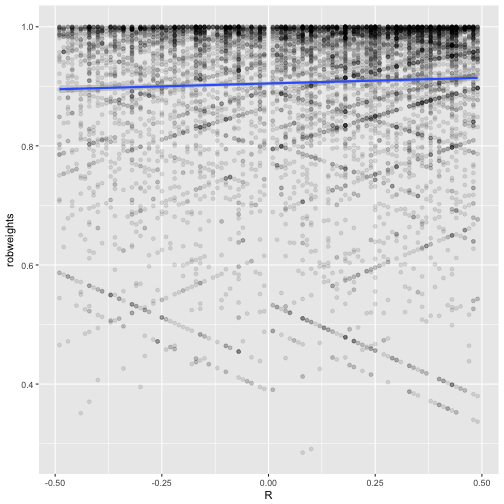
\includegraphics[width=0.9\textwidth]{graphics/weightPlot.png}
% \caption{A plot of robustness weights from our main analysis.}
% \label{fig:robweights}
% \end{figure}



% {\small
% \bibliographystyle{asa}
% \bibliography{./causalinference}
% }

% \end{document}

% \marginpar{Revisit after revisiting $N_{j} \in \mathcal{F}^{*}$}
% Similarly, for asymptotic analysis of $t_e(\mathbf{Y}_H,\mathbf{R})$
% in RDDs we shall posit a triangular array of i.i.d. random vectors
% $\{(Y_{Ti(n)}, Y_{Ci(n)}, D_{Ti(n)}, D_{Ci(n)}, R_{i(n)}): i=1,
% \ldots, n; n\}$, with $Z_{i(n)} \equiv \indicator{R_{i(n)} \leq 0}$ as
% otherwise; before more discussion of this, however, we establish a
% basic property of $t_{u}$ under conditioning on $\mathcal{N}_{\infty}$.

